% =====================================================================
%  5.1 Sinus, cosinus og tangens — teori og oppgaver
% =====================================================================

\del{1}{Sinus, cosinus og tangens i rettvinklede trekanter}

\begin{ordliste}
hypotenus & Den lengste siden i en rettvinklet trekant. Den ligger rett overfor den rette vinkelen. & \mittsprak\\
motstående katet & Kateten som ligger rett overfor vinkelen $v$. & \mittsprak\\
hosliggende katet & Kateten som ligger inntil vinkelen $v$ (ved siden av den). & \mittsprak\\
sinus, cosinus, tangens & Tre forhold mellom sidene i en rettvinklet trekant. De skrives $\sin v$, $\cos v$ og $\tan v$. & \mittsprak\\
\end{ordliste}

\begin{mustkunne}
\begin{minipage}[t]{0.50\linewidth}
\textbf{Definisjon.} For en spiss vinkel $v$ i en rettvinklet trekant er
\[ \sin v = \frac{\text{motstående}}{\text{hypotenus}} \qquad
   \cos v = \frac{\text{hosliggende}}{\text{hypotenus}} \qquad
   \tan v = \frac{\text{motstående}}{\text{hosliggende}} \]
\textbf{Hvorfor bare vinkelen betyr noe.} To rettvinklede trekanter med samme vinkel $v$ er formlike. Da er forholdet mellom to sider likt i begge: $\frac{1,5}{2,5} = \frac{3}{5}$ i figuren.
Derfor kan kalkulatoren gi $\sin v$ ut fra $v$ alene.\par
\textbf{Kalkulatoren} må stå i grader (DEG), ikke radianer (RAD).
Finn vinkelen med $\sin^{-1}$, $\cos^{-1}$ eller $\tan^{-1}$.
\end{minipage}\hfill
\begin{minipage}[t]{0.46\linewidth}
\centering
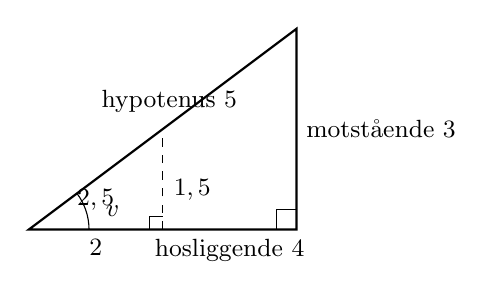
\begin{tikzpicture}[baseline=(current bounding box.north),scale=0.85,font=\small]
  \draw[thick] (0,0)--(4,0)--(4,3)--cycle;
  \draw[dashed] (2,0)--(2,1.5);
  \draw (3.7,0)--(3.7,0.3)--(4,0.3);
  \draw (1.8,0)--(1.8,0.2)--(2,0.2);
  \draw (0.9,0) arc (0:36.87:0.9);
  \node at (1.25,0.27) {$v$};
  \node[below] at (1,0) {$2$};
  \node[below] at (3,0) {hosliggende $4$};
  \node[right] at (4,1.5) {motstående $3$};
  \node[sloped,above] at (2.1,1.6) {hypotenus $5$};
  \node[sloped,below] at (1,0.75) {$2,5$};
  \node[right] at (2.02,0.6) {$1,5$};
\end{tikzpicture}
\end{minipage}
\end{mustkunne}

\begin{eksempel}[1 — finn en katet]
I en rettvinklet trekant er hypotenusen $8,0$ cm og $v = 28^\circ$. Finn den motstående kateten $x$. Svar med én desimal.

\begin{stegtabell}
$\sin 28^\circ = \dfrac{x}{8,0}$ & Motstående og hypotenus hører til sinus.\\
$x = 8,0 \cdot \sin 28^\circ$ & Gang med $8,0$ på begge sider.\\
$x \approx 3,8$ cm & Kalkulatoren står i DEG.\\
Kontroll: & Kateten er kortere enn hypotenusen $8,0$ cm. Det stemmer.\\
\end{stegtabell}
\end{eksempel}

\begin{eksempel}[2 — finn en vinkel]
I en rettvinklet trekant er motstående katet $5,0$ og hosliggende katet $7,0$. Finn $v$. Svar med én desimal.

\begin{stegtabell}
$\tan v = \dfrac{5,0}{7,0}$ & Motstående og hosliggende hører til tangens.\\
$v = \tan^{-1}\!\left(\dfrac{5,0}{7,0}\right)$ & Bruk $\tan^{-1}$ for å gå fra forholdet til vinkelen.\\
$v \approx 35,5^\circ$ & Kalkulatoren står i DEG.\\
Kontroll: & $\tan 35,5^\circ \approx 0,71$ og $\frac{5,0}{7,0} \approx 0,71$. Det stemmer.\\
\end{stegtabell}
\end{eksempel}

\begin{vanligfeil}
\begin{itemize}[leftmargin=1.2em,itemsep=1pt,topsep=0pt]
  \item $\cos v = \frac{\text{hypotenus}}{\text{hosliggende}}$ er feil. Hypotenusen står alltid nederst for $\sin v$ og $\cos v$: $\cos v = \frac{\text{hosliggende}}{\text{hypotenus}}$.
  \item Kalkulatoren står i RAD. Da gir $\sin 30$ svaret $-0,988$ og ikke $0,5$. Sjekk at det står DEG.
  \item $\sin^{-1} x = \frac{1}{\sin x}$ er feil. $\sin^{-1}$ finner vinkelen: $\sin^{-1}(0,5) = 30^\circ$, mens $\frac{1}{\sin 30^\circ} = 2$.
  \item Definisjonene gjelder ikke generelt i en trekant uten rett vinkel. Det finnes ingen hypotenus der.
\end{itemize}
\end{vanligfeil}

\nivaahode{1}

\oppg{1.1}{1}{\uh}
\begin{minipage}[t]{0.58\linewidth}
Figuren viser en rettvinklet trekant. Skriv $\sin v$, $\cos v$ og $\tan v$ som brøker.
\end{minipage}\hfill
\begin{minipage}[t]{0.38\linewidth}
\centering
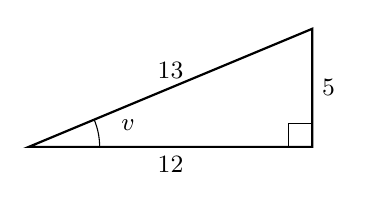
\begin{tikzpicture}[baseline=(current bounding box.north),scale=0.3,font=\small]
  \draw[thick] (0,0)--(12,0)--(12,5)--cycle;
  \draw (11,0)--(11,1)--(12,1);
  \draw (3,0) arc (0:22.6:3);
  \node at (4.2,0.9) {$v$};
  \node[below] at (6,0) {$12$};
  \node[right] at (12,2.5) {$5$};
  \node[sloped,above] at (6,2.5) {$13$};
\end{tikzpicture}
\end{minipage}

\oppg{1.2}{1}{\uh}
I en rettvinklet trekant er hypotenusen $15$ og $\sin v = 0,8$. Fullfør.
\begin{tasks}(1)
  \task Motstående katet: $\sin v = \dfrac{\text{motstående}}{15}$, så motstående $= \skrivlinje[2cm] \cdot 15 = \skrivlinje[2cm]$.
  \task Finn hosliggende katet med Pytagoras.
  \task Finn $\cos v$ som uforkortet brøk, og forkort den.
\end{tasks}

\oppg{1.3}{1}{\mh}
Sett kalkulatoren i DEG. Regn ut.
\begin{tasks}(2)
  \task $\sin 25^\circ$ (tre desimaler)
  \task $\cos 64^\circ$ (tre desimaler)
  \task $\tan 55^\circ$ (tre desimaler)
  \task $v$ når $\tan v = 2$ (én desimal)
\end{tasks}

\nivaahode{2}

\oppg{1.4}{2}{\uh}
En rettvinklet trekant har kateter med lengde $9$ og $40$. Vinkelen $v$ ligger rett overfor kateten med lengde $9$.
\begin{tasks}(2)
  \task Finn hypotenusen.
  \task Finn $\sin v$, $\cos v$ og $\tan v$.
\end{tasks}

\oppg{1.5}{2}{\mh}
I en rettvinklet trekant er $v$ en av de spisse vinklene. Finn den ukjente siden. Svar med én desimal.
\begin{tasks}(1)
  \task $v = 37^\circ$ og hypotenusen er $12,0$ cm. Finn hosliggende katet.
  \task $v = 42^\circ$ og hosliggende katet er $9,0$ cm. Finn motstående katet.
  \task $v = 33^\circ$ og motstående katet er $5,5$ cm. Finn hypotenusen.
\end{tasks}

\oppg{1.6}{2}{\mh}
En stige er $5,0$ m lang. Den står mot en loddrett vegg, og foten står $1,5$ m fra veggen. Tegn en skisse.
\begin{tasks}(1)
  \task Finn vinkelen mellom stigen og bakken. Svar med én desimal.
  \task Finn hvor høyt opp på veggen stigen når. Svar med én desimal.
\end{tasks}

\oppg{1.7}{2}{\mh}
Eleven skal finne hosliggende katet $x$ når hypotenusen er $14$ og $v = 40^\circ$. Finn \textbf{den første feilen}. Løs riktig.
\[ \cos 40^\circ = \frac{x}{14} \quad\longrightarrow\quad x = 14 \cdot \cos 40^\circ \quad\longrightarrow\quad x = 14 \cdot (-0,667) \quad\longrightarrow\quad x = -9,3 \]

\nivaahode{3}

\oppg{1.8}{3}{\uh}
Anta at $v$ er en spiss vinkel i en rettvinklet trekant. Er påstanden alltid, noen ganger eller aldri sann? Begrunn svaret.
\begin{tasks}(3)
  \task $\sin v < 1$
  \task $\tan v < 1$
  \task $\sin v + \cos v = 1$
\end{tasks}

\oppg{1.9}{3}{\uh}
Vis at $\tan v = \dfrac{\sin v}{\cos v}$ i en rettvinklet trekant. Forklar hver overgang.

\oppg{1.10}{3}{\uh}
Finn sidene i en rettvinklet trekant der $\tan v = \dfrac{7}{24}$ og hypotenusen er $50$. Forklar hvorfor det finnes bare én slik trekant.

\begin{sjekk}
\begin{tasks}(2)
  \task En rettvinklet trekant har motstående katet $7$ og hypotenus $25$. Finn $\cos v$.
  \task Regn ut $\sin 50^\circ$ med to desimaler.
  \task! Hvorfor er $\sin v$ den samme i en stor og en liten rettvinklet trekant med samme $v$?
\end{tasks}
\end{sjekk}

% ---------------------------------------------------------------------

\del{2}{Eksakte verdier og enhetssirkelen}

\begin{ordliste}
eksakt verdi & Svaret skrevet med rottegn og brøk, uten avrunding. For eksempel $\frac{\sqrt2}{2}$. & \mittsprak\\
enhetssirkel & Sirkelen med sentrum i origo og radius 1. & \mittsprak\\
spiss vinkel & En vinkel mellom $0^\circ$ og $90^\circ$. & \mittsprak\\
stump vinkel & En vinkel mellom $90^\circ$ og $180^\circ$. & \mittsprak\\
\end{ordliste}

\begin{mustkunne}
\begin{minipage}[t]{0.50\linewidth}
\textbf{Eksakte verdier.} Et halvt kvadrat med side 1 har diagonal $\sqrt2$. Da er $\sin 45^\circ = \frac{1}{\sqrt2} = \frac{\sqrt2}{2}$ (utvid med $\sqrt2$).
\par\smallskip
\renewcommand{\arraystretch}{1.4}
\begin{tabular}[t]{@{}c|c c c@{}}
$v$ & $30^\circ$ & $45^\circ$ & $60^\circ$\\\hline
$\sin v$ & $\frac{1}{2}$ & $\frac{\sqrt2}{2}$ & $\frac{\sqrt3}{2}$\\
$\cos v$ & $\frac{\sqrt3}{2}$ & $\frac{\sqrt2}{2}$ & $\frac{1}{2}$\\
$\tan v$ & $\frac{\sqrt3}{3}$ & $1$ & $\sqrt3$\\
\end{tabular}
\par\smallskip
\textbf{Pytagoras gir} $a^2 + b^2 = c^2$. Del med $c^2$:
\[ \sin^2 v + \cos^2 v = 1 \]
\end{minipage}\hfill
\begin{minipage}[t]{0.46\linewidth}
\textbf{Enhetssirkelen.} For $0^\circ \le v \le 180^\circ$ er $(\cos v,\ \sin v)$ koordinatene til punktet $P$ på sirkelen. Trekanten inni sirkelen har hypotenus 1, så for spisse $v$ gir det samme svar som før.
\par\smallskip
\centering
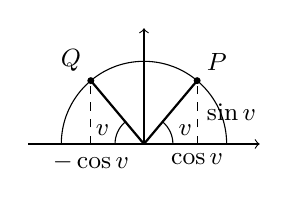
\begin{tikzpicture}[baseline=(current bounding box.north),scale=1.05,font=\small]
  \draw[->] (-1.4,0)--(1.4,0);
  \draw[->] (0,0)--(0,1.4);
  \draw (1,0) arc (0:180:1);
  \draw[thick] (0,0)--(0.643,0.766);
  \draw[thick] (0,0)--(-0.643,0.766);
  \draw[dashed] (0.643,0)--(0.643,0.766);
  \draw[dashed] (-0.643,0)--(-0.643,0.766);
  \fill (0.643,0.766) circle (1.2pt) node[above right] {$P$};
  \fill (-0.643,0.766) circle (1.2pt) node[above left] {$Q$};
  \draw (0.35,0) arc (0:50:0.35);
  \node at (0.5,0.17) {$v$};
  \draw (-0.35,0) arc (180:130:0.35);
  \node at (-0.5,0.17) {$v$};
  \node[below] at (0.643,0) {$\cos v$};
  \node[below] at (-0.643,0) {$-\cos v$};
  \node[right] at (0.643,0.38) {$\sin v$};
\end{tikzpicture}
\par\smallskip
\raggedright
Symmetri om $y$-aksen gir for stumpe vinkler ($Q$ har vinkel $180^\circ - v$):
\[ \sin(180^\circ - v) = \sin v \qquad \cos(180^\circ - v) = -\cos v \]
\end{minipage}
\end{mustkunne}

\begin{eksempel}[1 — utled $\sin 60^\circ$]
Utled $\sin 60^\circ$ fra en likesidet trekant med side 2. Alle vinklene er $60^\circ$. Vi halverer trekanten med en høyde $h$.

\begin{minipage}[t]{0.66\linewidth}
\begin{stegtabell}
Rettvinklet trekant med hypotenus $2$, kortkatet $1$ og vinkel $60^\circ$. & Høyden deler grunnlinjen i to like deler.\\
$h^2 + 1^2 = 2^2$ & Pytagoras.\\
$h = \sqrt3$ & Høyden er den ukjente kateten.\\
$\sin 60^\circ = \dfrac{h}{2} = \dfrac{\sqrt3}{2}$ & Motstående katet delt på hypotenus.\\
\end{stegtabell}
\end{minipage}\hfill
\begin{minipage}[t]{0.30\linewidth}
\centering
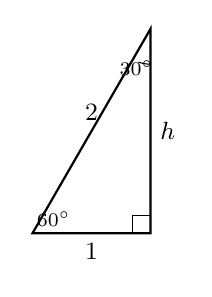
\begin{tikzpicture}[baseline=(current bounding box.north),scale=1.5,font=\small]
  \draw[thick] (0,0)--(1,0)--(1,1.732)--cycle;
  \draw (0.85,0)--(0.85,0.15)--(1,0.15);
  \draw (1,1.732) ++(250:0.3) arc (250:270:0.3);
  \node at (0.88,1.4) {\scriptsize$30^\circ$};
  \node at (0.18,0.12) {\scriptsize$60^\circ$};
  \node[below] at (0.5,0) {$1$};
  \node[right] at (1,0.87) {$h$};
  \node[sloped,above] at (0.5,0.87) {$2$};
\end{tikzpicture}
\end{minipage}
\end{eksempel}

\begin{eksempel}[2 — stump vinkel]
Finn $\sin 150^\circ$ og $\cos 150^\circ$ eksakt.

\begin{stegtabell}
$150^\circ = 180^\circ - 30^\circ$ & Skriv vinkelen som $180^\circ - v$ med spiss $v$.\\
$\sin 150^\circ = \sin 30^\circ = \dfrac{1}{2}$ & $\sin(180^\circ - v) = \sin v$.\\
$\cos 150^\circ = -\cos 30^\circ = -\dfrac{\sqrt3}{2}$ & $\cos(180^\circ - v) = -\cos v$.\\
Kontroll: $\left(\frac12\right)^2 + \left(-\frac{\sqrt3}{2}\right)^2 = \frac14 + \frac34 = 1$ & Stemmer med $\sin^2 v + \cos^2 v = 1$.\\
\end{stegtabell}
\end{eksempel}

\begin{vanligfeil}
\begin{itemize}[leftmargin=1.2em,itemsep=1pt,topsep=0pt]
  \item $\sin(2v) = 2\sin v$ gjelder ikke generelt. For $v = 30^\circ$ er $\sin 60^\circ = \frac{\sqrt3}{2}$, men $2 \sin 30^\circ = 1$.
  \item $\sin v = 0,5$ har bare løsningen $30^\circ$ er feil. Mellom $0^\circ$ og $180^\circ$ er både $30^\circ$ og $150^\circ$ løsninger.
  \item $\cos(180^\circ - v) = \cos v$ er feil. Riktig er $\cos(180^\circ - v) = -\cos v$. For eksempel er $\cos 150^\circ$ negativ.
\end{itemize}
\end{vanligfeil}

\nivaahode{1}

\oppg{2.1}{1}{\uh}
Bruk tabellen. Svar eksakt.
\begin{tasks}(4)
  \task $\sin 30^\circ$
  \task $\cos 60^\circ$
  \task $\tan 45^\circ$
  \task $\cos 45^\circ$
\end{tasks}

\oppg{2.2}{1}{\uh}
I en rettvinklet trekant er $v = 30^\circ$ og hypotenusen er $14$. Finn begge katetene eksakt.

\oppg{2.3}{1}{\uh}
Bruk enhetssirkelen. Hva er
\begin{tasks}(4)
  \task $\cos 0^\circ$
  \task $\sin 90^\circ$
  \task $\cos 180^\circ$
  \task $\sin 180^\circ$
\end{tasks}

\nivaahode{2}

\oppg{2.4}{2}{\uh}
Finn eksakt verdi.
\begin{tasks}(4)
  \task $\sin 120^\circ$
  \task $\sin 135^\circ$
  \task $\cos 135^\circ$
  \task $\cos 120^\circ$
\end{tasks}

\oppg{2.5}{2}{\mh}
Finn alle vinkler $v$ mellom $0^\circ$ og $180^\circ$. Svar med én desimal.
\begin{tasks}(3)
  \task $\sin v = 0,8$
  \task $\cos v = -0,25$
  \task $\sin v = 0,92$
\end{tasks}

\oppg{2.6}{2}{\uh}
Marit påstår at $\sin(2v) = 2\sin v$.
\begin{tasks}(1)
  \task Sett inn $v = 45^\circ$ og regn eksakt. Hva viser det?
  \task Finn en vinkel der påstanden likevel stemmer.
\end{tasks}

\oppg{2.7}{2}{\mh}
Vinkelen $v$ er stump og $\sin v = \dfrac{8}{17}$. Eleven regner slik:
\begin{align*}
&\sin^2 v + \cos^2 v = 1\\
&\cos^2 v = 1 - \left(\tfrac{8}{17}\right)^2 = \tfrac{225}{289}\\
&\cos v = \tfrac{15}{17}\\
&v = \cos^{-1}\!\left(\tfrac{15}{17}\right) \approx 28,1^\circ
\end{align*}
Finn \textbf{den første feilen}. Finn riktig $\cos v$ og riktig $v$ (én desimal).

\nivaahode{3}

\oppg{2.8}{3}{\uh}
Anta at $0^\circ \le v \le 180^\circ$. Er påstanden alltid, noen ganger eller aldri sann? Begrunn med enhetssirkelen.
\begin{tasks}(1)
  \task $\cos v > 0$
  \task $\sin v = \cos v$
  \task To ulike vinkler mellom $0^\circ$ og $180^\circ$ har samme cosinusverdi.
\end{tasks}

\oppg{2.9}{3}{\uh}
To vinkler $v_1$ og $v_2$ i samme trekant har $\sin v_1 = \sin v_2$. Hva kan du si om $v_1$ og $v_2$? Forklar.

\begin{sjekk}
\begin{tasks}(2)
  \task Skriv $\tan 60^\circ$ eksakt.
  \task Finn alle $v$ mellom $0^\circ$ og $180^\circ$ med $\sin v = \frac{\sqrt3}{2}$.
  \task! Hvorfor er $\sin^2 100^\circ + \cos^2 100^\circ = 1$? Forklar med enhetssirkelen.
\end{tasks}
\end{sjekk}
